\newpage
\section{Thiết bị và thông số kỹ thuật}

\subsection{Mạch điều khiển trung tâm Yolo:Bit}
Yolo:Bit là máy tính nhúng dựa trên chip ESP32, hỗ trợ WiFi, bluetooth và chạy MicroPython. Mạch được thiết kế an toàn (3.3V), tích hợp nhiều cảm biến và chân cắm mở rộng, tối ưu cho các ứng dụng IoT.

\begin{figure}[H]
    \centering
    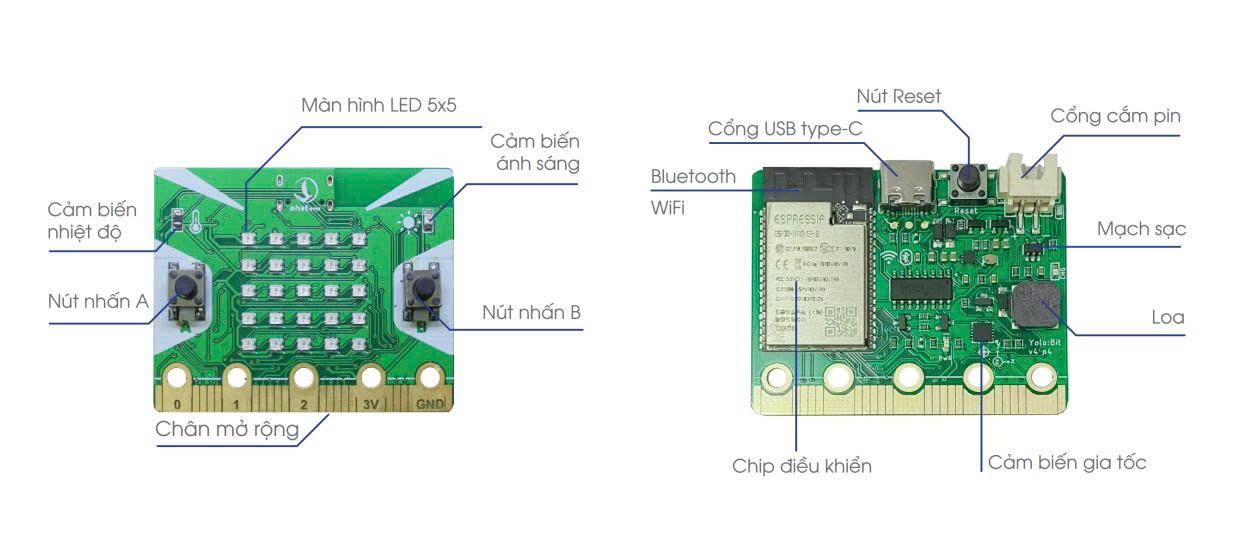
\includegraphics[width=0.6\textwidth]{img/YOLObit.png}
    \caption{Mạch Yolo:Bit và sơ đồ chân cắm}
\end{figure}

\textbf{Thông số cơ bản:} RAM 8MB, Flash 4MB, vi xử lý lõi kép ESP32, kích thước 4x5cm.

\subsection{Hệ thống thiết bị ngoại vi}

\subsubsection{Thiết bị kết nối}
\begin{itemize}
    \item \textbf{Mạch mở rộng Grove shield:} Cung cấp 9 cổng cắm chuẩn grove (P0-P2, I2C, UART), giúp kết nối các module nhanh chóng mà không cần hàn mạch.
    \item \textbf{Module đóng ngắt 2 kênh:} Đóng vai trò relay, chuyển đổi tín hiệu điều khiển để bật/tắt các thiết bị dùng cổng USB như máy bơm hoặc đèn LED.
\end{itemize}

\begin{figure}[H]
    \centering
    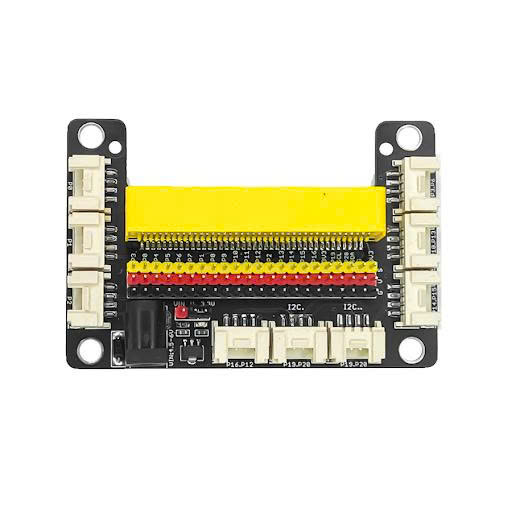
\includegraphics[width=0.4\textwidth]{img/Mạch mở rộng YoloBit.png}
    \caption{Grove shield và module đóng ngắt}
\end{figure}

\subsubsection{Cảm biến (input)}
\begin{itemize}
    \item \textbf{DHT20:} Đo nhiệt độ (-40 đến +80 \textdegree C) và độ ẩm không khí (0--100\%) qua giao thức I2C.
    \item \textbf{Độ ẩm đất:} Trả về giá trị analog giúp xác định tình trạng khô/ướt của đất để điều khiển tưới.
    \item \textbf{Ánh sáng và PIR:} Quang trở đo cường độ sáng và cảm biến hồng ngoại phát hiện chuyển động trong phạm vi 6m.
\end{itemize}

\subsubsection{Thiết bị chấp hành (output)}
\begin{itemize}
    \item \textbf{Màn hình LCD 1602 I2C:} Hiển thị trực quan các thông số môi trường và trạng thái hệ thống (2 dòng, 16 ký tự).
    \item \textbf{Hệ thống tưới và chiếu sáng:} Gồm máy bơm mini (tưới nước) và module 4 LED RGB WS2812 (chiếu sáng/cảnh báo), điều khiển thông qua Yolo:Bit.
\end{itemize}

\subsubsection{Các thiết bị liên quan khác}
\begin{figure}[H]
    \centering
    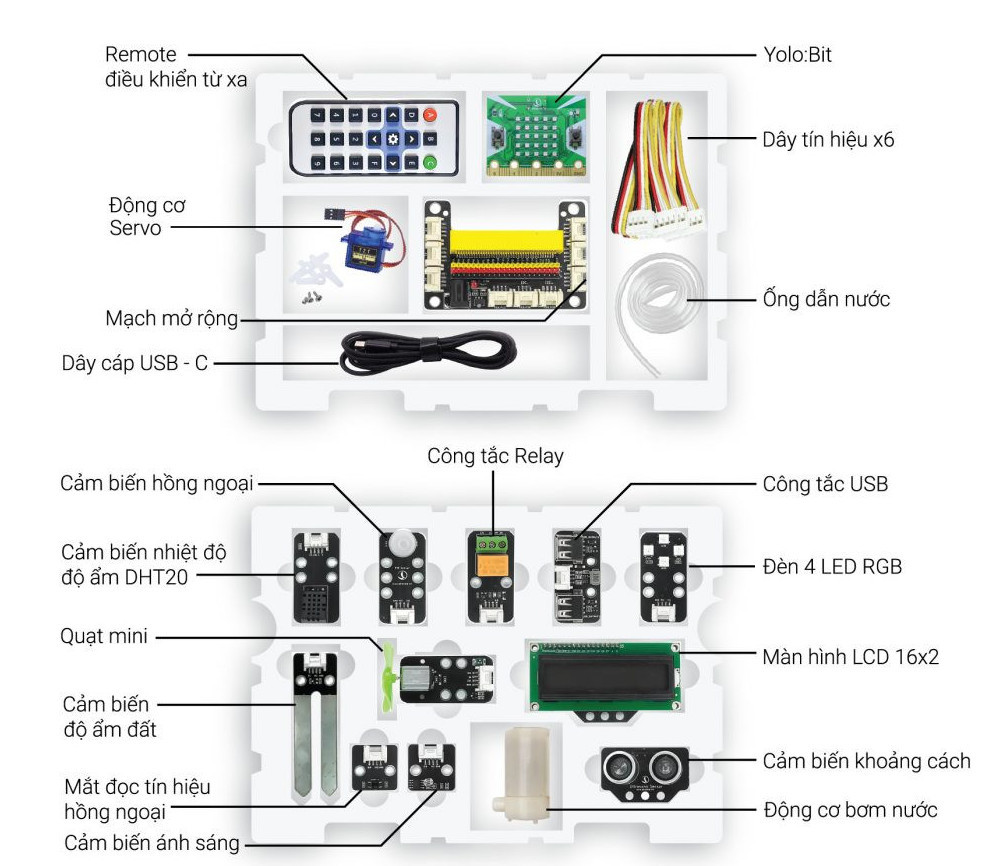
\includegraphics[width=0.8\textwidth]{img/device_list.png}
    \caption{Danh sách các thiết bị liên quan}
\end{figure}
